\documentclass{article}
\usepackage[utf8]{inputenc}
\usepackage{graphicx}
\usepackage{pgfgantt}
\usepackage{lscape}
\usepackage{rotating}
\renewcommand{\refname}{Kaynakça}
\usepackage{pdflscape}
\usepackage{hyperref}

\begin{document}

\begin{titlepage}
    \centering
    %\vspace*{0.5cm}
    
\includegraphics[width=0.2\textwidth]{ksbu.png} % Logonuzun olduğu dosya adını buraya girin
    \vskip 1em
    \vspace{1cm}
    {\scshape\Large Reinforcement Learning Tekniğini Kullanarak Yapay Zeka Tarafından Yönetilen Bir Arabaya Pisti Tamamlatmak \par}
    \vspace{1cm}
    {\medium Yazar: Mert Koca \par}
    {\medium \today\par}
    %\vfill
    \begin{center}
        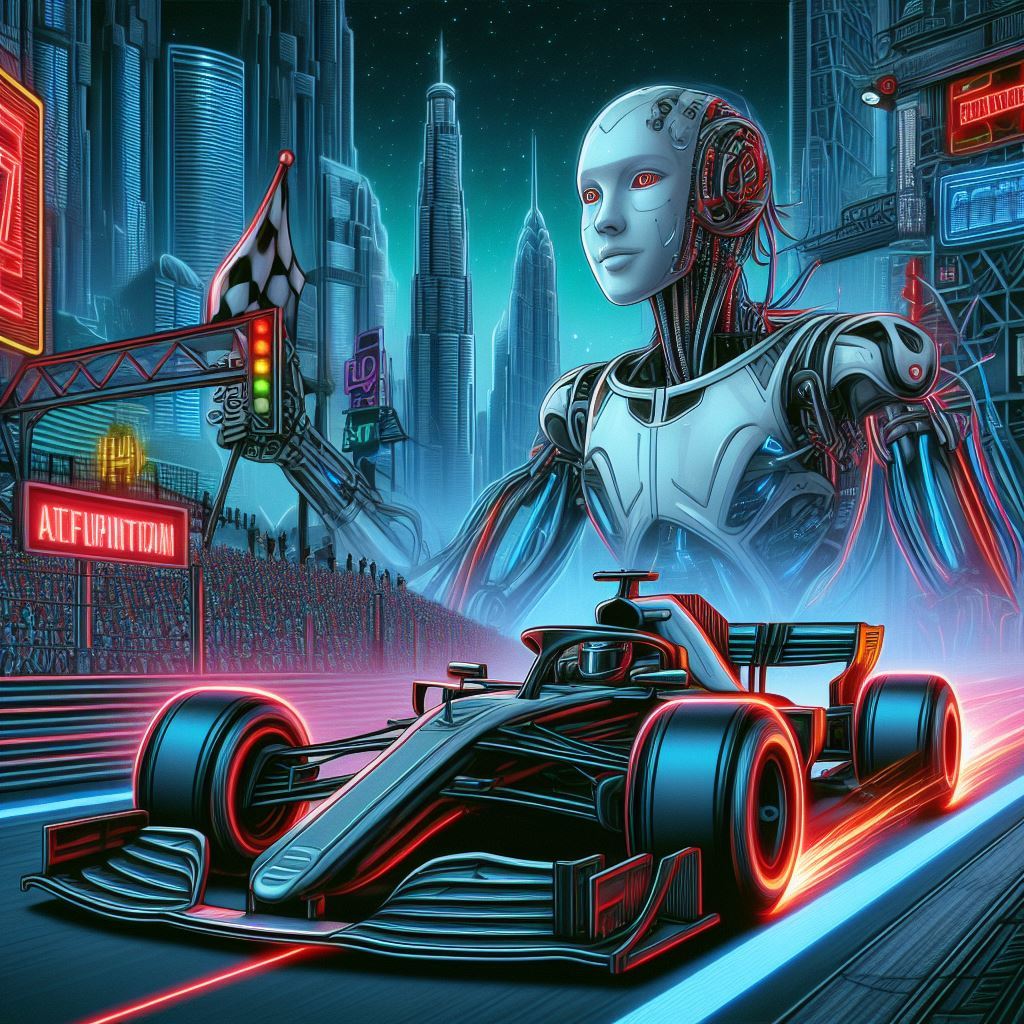
\includegraphics[width=0.5\textwidth]{f1ai.jpeg} % Araba resminin dosya adını belirtin
    \end{center}
    \vspace{0.5cm}
    {\medium Özet \par}
    \vspace{0.1cm}
    {Bu proje, yapay zeka kullanarak bir arabanın otomatik olarak bir pisti tamamlamasını sağlamayı hedefler. Yapay zeka, görsel girdi olarak pistin haritasını alacak ve aracı uygun şekilde yönlendirerek pisti en kısa sürede tamamlamaya çalışacak. Bu projede reinforcement learning (teşvik öğrenimi) algoritması kullanılarak gerçekleştirilecek. Proje, yapay zeka temelli oyun geliştirme, teşvik öğrenimi ve simülasyon gibi alanlara odaklanacak.\par}
    \vspace{1cm}
\end{titlepage}
\newpage

\section{Giriş}
\rule{\textwidth}{0.5pt}
Reinforcement learning algoritması, bir ajanın çevresiyle etkileşime geçerek deneyimlerinden öğrenmesini sağlar ve bu öğrenme sürecini en iyi şekilde nasıl yönlendireceğini belirler. Araba yarışı, özellikle karmaşık çevrelerde hızlı ve doğru kararlar gerektiren bir projedir. Bu proje, reinforcement learning'in gücünü araç yarışı simülasyonlarıyla birleştirerek, bir aracın yarış pistinde optimum performansı elde etmesi için nasıl öğrenebileceğini araştırmayı amaçlamaktadır. Bu projenin başarısı, gerçek dünya uygulamalarında otonom araçların geliştirilmesi gibi birçok alana ilham verebilir.\\[15pt]

\section{Literatür Çalışması}
\rule{\textwidth}{0.5pt}
Ibrahim Sobh Ibrahim'in yürüttüğü araştırma\cite{kiran2021deep}, Reinforcement Learning (RL) algoritmalarını kullanarak ajanların dinamik ortamlarda hızlı bir şekilde öğrenmesini ve adapte olmasını vurgulamaktadır. Derin RL'yi kullanarak, çalışma, özellikle müzakere gerektiren ve dinamik etkileşimler gerektiren senaryolarda otonom ajanların karar verme yeteneklerini artırmayı amaçlamaktadır.\\[5pt]
\newline
Ayrıca, çalışma, RL ajanlarının öğrenme sürecini yönlendirmek için etkili ödül fonksiyonlarının tasarlanmasının önemini vurgulamaktadır. Literatürde tartışıldığı gibi, ödül şekillendirme, istenen davranışlara dayalı olarak ajanlara ek rehberlik sağlayarak öğrenme sürecini hızlandırmada kritik bir rol oynamaktadır. Bu yaklaşım, ajanların ortamla etkileşimler yoluyla kümülatif ödülleri maksimize etmeye çalıştığı RL'nin temel prensibiyle uyumludur.
\\[5pt]
\newline
Son yıllarda derin öğrenme ve özellikle de Derin Pekiştirmeli Öğrenme (DPO) alanındaki ilerlemeler\cite{sallab2017deep}, otonom sürüş sistemlerinin geliştirilmesinde önemli bir rol oynamaktadır. El Sallab ve diğerleri (2017), otonom sürüş için bir Derin Pekiştirmeli Öğrenme çerçevesi önermişlerdir. Bu çerçeve, Reküran Sinir Ağları (RSA) ve dikkat modellerini içererek karmaşık sürüş senaryolarıyla başa çıkmakta ve hesaplama karmaşıklığını azaltmaktadır. Araştırmacılar, bu çerçevenin TORCS simülatöründe test edildiğini ve başarılı öğrenme sonuçları elde edildiğini belirtmektedirler. Ayrıca, önerilen çerçeve, RNN'leri kısmen gözlemlenebilir senaryoları ele almak için entegre etmektedir. Bu çalışma, otonom sürüş sistemlerinin geliştirilmesinde derin öğrenme tekniklerinin etkili bir şekilde kullanılmasını vurgulamaktadır.\\[15pt]

\newpage
\newline
\noindent
flyyufelix adlı github kullanıcısının yaptığı "donkeyrl" projesinde Donkey Car adı verilen bir arabanın bir pist etrafında RL kullanarak kendi kendine dönmesini sağlamıştır. Bu projede Double Deep Q Learning (DDQN) kullanılmıştır. DDQN, bir ajanın çevresiyle etkileşime girerek belirli bir durumda alabileceği eylemler arasında en uygun olanını seçmeyi öğrenen bir güçlendirme öğrenme algoritmasıdır. Bunu, bir Q-değer fonksiyonu kullanılarak gerçekleştirilir. Q-değer fonksiyonu, bir durum ve bir eylem çifti için beklenen toplam ödülü temsil eder.\\[15pt]

\section{Yöntemler}
\rule{\textwidth}{0.5pt}
Bu projede, reinforcement learning algoritmalarını kullanarak bir aracın yarış pistinde optimal performansı öğrenmesini sağlamak için bir metodoloji izlenecektir. İlk olarak, yarış simülasyonu için uygun bir ortam oluşturulacak ve aracın bu ortamda hareket etmesi sağlanacaktır. Daha sonra, aracın davranışlarını kontrol etmek için bir reinforcement learning algoritması seçilecek ve bu algoritma modeli, aracın çevresini algılamasını ve çevresel faktörlere tepki vermesini sağlayacak şekilde ayarlanacaktır. Ardından, aracın deneyimlerinden öğrenerek, yarış pistinde en iyi performansı elde etmesini sağlamak için algoritma sürekli olarak güncellenecek ve iyileştirilecektir. Son olarak, algoritmanın eğitimi tamamlandıktan sonra, aracın gerçek zamanlı olarak yarış pistinde nasıl davrandığını test etmek için simülasyonlar üzerinde çeşitli denemeler yapılacak ve sonuçlar analiz edilecektir. Bu metodoloji, reinforcement learning'in araç yarışı gibi karmaşık görevlerde nasıl başarılı bir şekilde uygulanabileceğini anlamak için bir çerçeve sağlayacaktır.\\[5pt]
\newline
Bu projeyi uygulamaya geçireceğim platform olarak Unity oyun motorunu seçtim. Arayüz kullanılabilirliği, uygulama anlaşılabilirliği açısından en iyi performansı elde eteceğimi düşünüyorum. Kodlama açısından C Sharp dilini kullanacağım için Unity içerisinde Visual Studio Code uygulamasını kullanacağım. Arabanın kontorlleri, zamanlayıcı gibi kodlama gerektiren kısımları burada kodlayacağım.\\[15pt]

\newpage

\section{Veri Odaklı Sistem Tasarımı}
\rule{\textwidth}{0.5pt}

\subsection{Veri Toplama ve İşleme Bileşeni}
Sensörler aracılığıyla pistin gerçek zamanlı haritasını oluşturacak verileri toplama.
Kullanılacak kamera veya diğer algılayıcılarla çevrenin görüntülerini toplama.
\subsection{Yapay Zeka ve Öğrenme Bileşeni}
Veri odaklı algoritma seçimi, Reinforcement Learning (teşvik öğrenimi) algoritması kullanılacak.
Modelin eğitilmesi: Toplanan veriler üzerinde modelin eğitilmesi, pisti tamamlama görevini öğrenmesi.
Modelin güncellenmesi: Sürekli olarak yeni verilerle modelin güncellenmesi ve iyileştirilmesi.
\subsection{Karar ve Yönlendirme Bileşeni:}
Model tarafından verilen kararların alınması ve işlenmesi.
Arabanın mevcut konumu ve pist haritası dikkate alınarak bir sonraki adımın belirlenmesi.
Arabanın hareketini yönlendirme: Hız, yönlendirme açısı vb. ayarlama.
\subsection{Simülasyon ve Test Bileşeni}
Geliştirilen sistemin simülasyon ortamında test edilmesi.
Farklı senaryolarda ve çevresel koşullarda sistemin performansının değerlendirilmesi.
Modelin güvenilirliğinin ve dayanıklılığının test edilmesi.
\subsection{Görselleştirme ve Raporlama Bileşeni}
Sistemin çalışmasıyla ilgili verilerin görselleştirilmesi.
Performans metriklerinin ve sonuçların raporlanması.
Karar vericilere veya paydaşlara sunumlar için raporlar hazırlama.\\[15pt]

\noindent Veri odaklı sistem tasarımı, bir sistemin geliştirilmesi veya iyileştirilmesi sürecinde veriye dayalı bir yaklaşımı benimseyen bir metodolojidir. Bu yaklaşım, karar alma süreçlerinin verilere dayandığı, performansın sürekli olarak izlendiği ve geri bildirimlerin değerlendirildiği bir çerçeve sunar.

\newpage

\section{Proje Aşamaları}
\rule{\textwidth}{0.5pt}

\subsection{Hazırlık ve Araştırma}
Teşvik öğrenimi ve reinforcement learning konseptleri incelenecek. Gerekli yazılım araçlarını ve kütüphaneleri (Unity, C Sharp, vs.) yüklenip yapılandırılacak. Basit bir araba simülasyonu oluşturulacak ve Unity'de çalışır hale getirilecek..\\[15pt]

\subsection{Ortam ve Veri Toplama}
Pistin çevresi ve düzeni gibi ortamı oluşturulacak. Veri toplama için bir veri toplama arayüzü oluşturulacak ve araba simülasyonunu bu arayüz üzerinden kullanarak veri toplanacak. Toplanan verileri düzenlenip işlenecek, uygun formatlara dönüştürülecek.\\[15pt]

\subsection{Teşvik Öğrenme Algoritmasının Uygulanması}
Seçilen bir teşvik öğrenme algoritması (örneğin, Q-learning, Deep Q-Networks, vs.) uygulanacak. Algoritma, veri kümesi üzerinde eğitilecek ve başlangıçta basit bir ortamda test edilecek. Algoritmanın performansını değerlendirilecek ve gerektiğinde ayarlamalar yapılacak.\\[15pt]

\subsection{Gelişmiş Simülasyon ve Ayarlamalar}
Daha karmaşık pistler, engeller ve dinamik ortamlar eklenecek. Teşvik öğrenme algoritması bu geliştirilmiş simülasyon üzerinde yeniden eğitilecek. Algoritmanın performansını iyileştirmek için parametreler ayarlanacak.\\[15pt]

\subsection{Son Dokunuşlar ve Değerlendirme}
Kullanıcı arayüzü eklenecek, gerektiğinde grafiksel iyileştirmeler yapılacak.
Proje test edilecek ve hata ayıklama yapılacak.
Sonuçları ve elde edilen son performans değerlendirilecek.
Projenin dokümantasyonunu hazırlanacak.\\[15pt]

\newpage

\begin{landscape}
\thispagestyle{empty}
    \begin{figure}
     \centering
  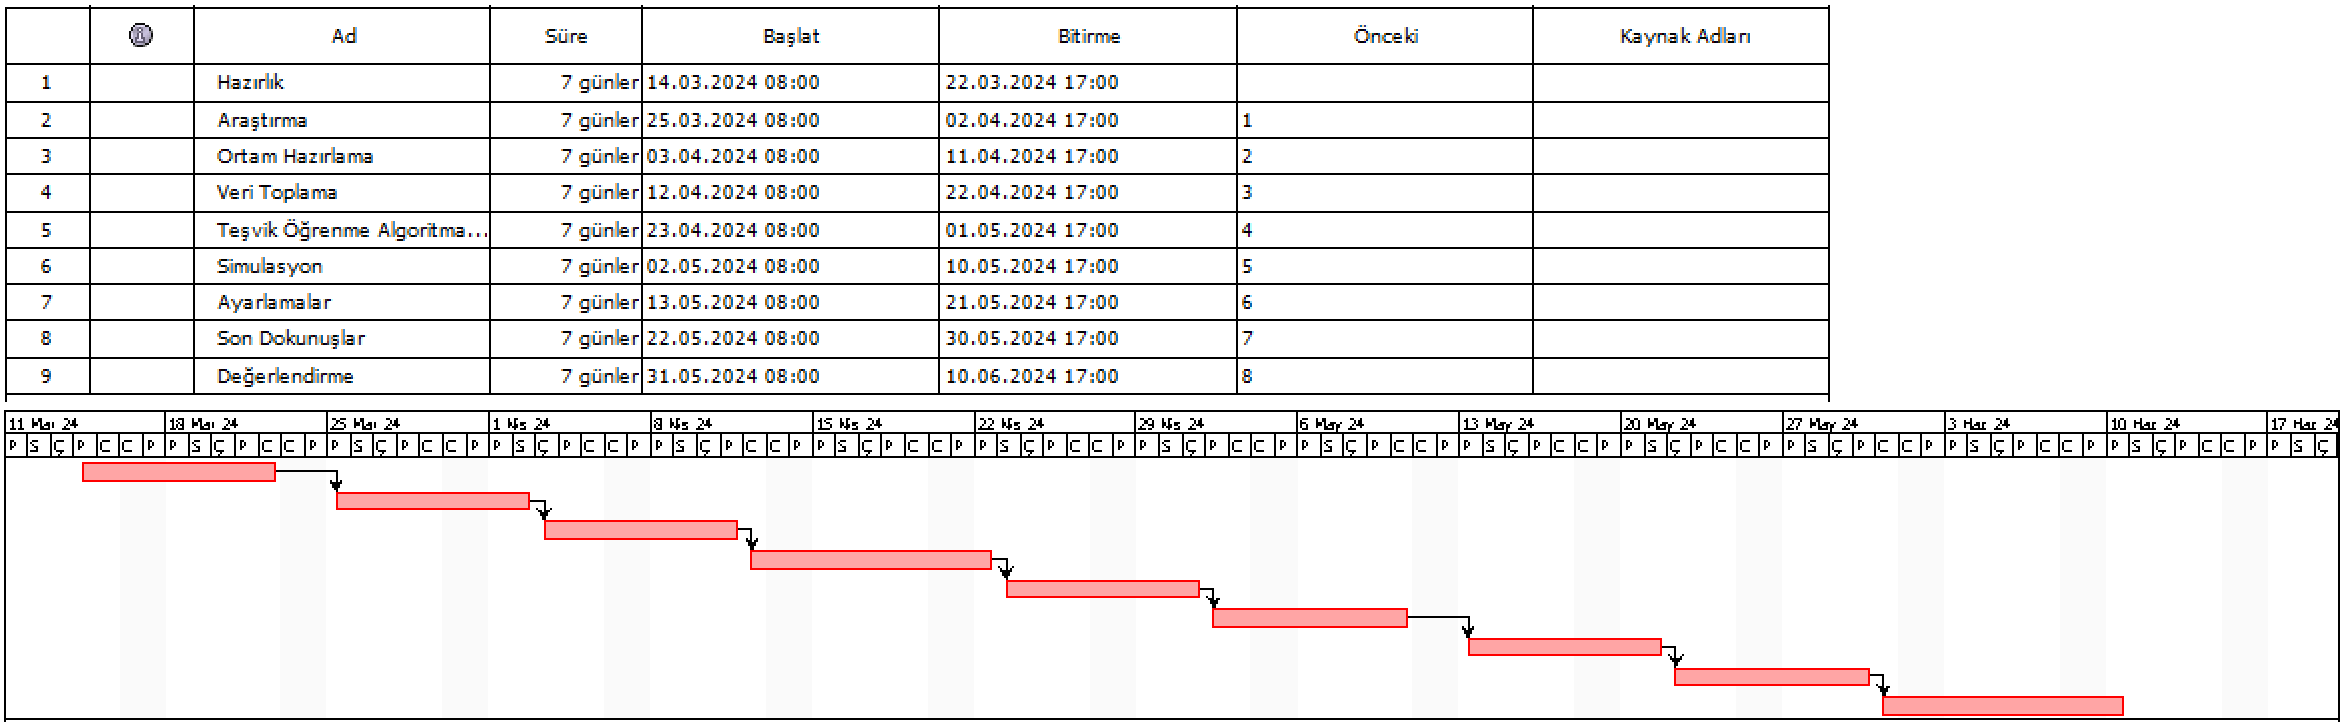
\includegraphics[width=1.8\textwidth]{Merged.png}\centering % Resim dosyasının adını ve uzantısını belirtin
  \caption{Gantt Chart}
  \label{fig:resim_etiketi}
\end{figure}

    % Yana çevirmek istediğiniz içerik buraya gelir
\end{landscape}


%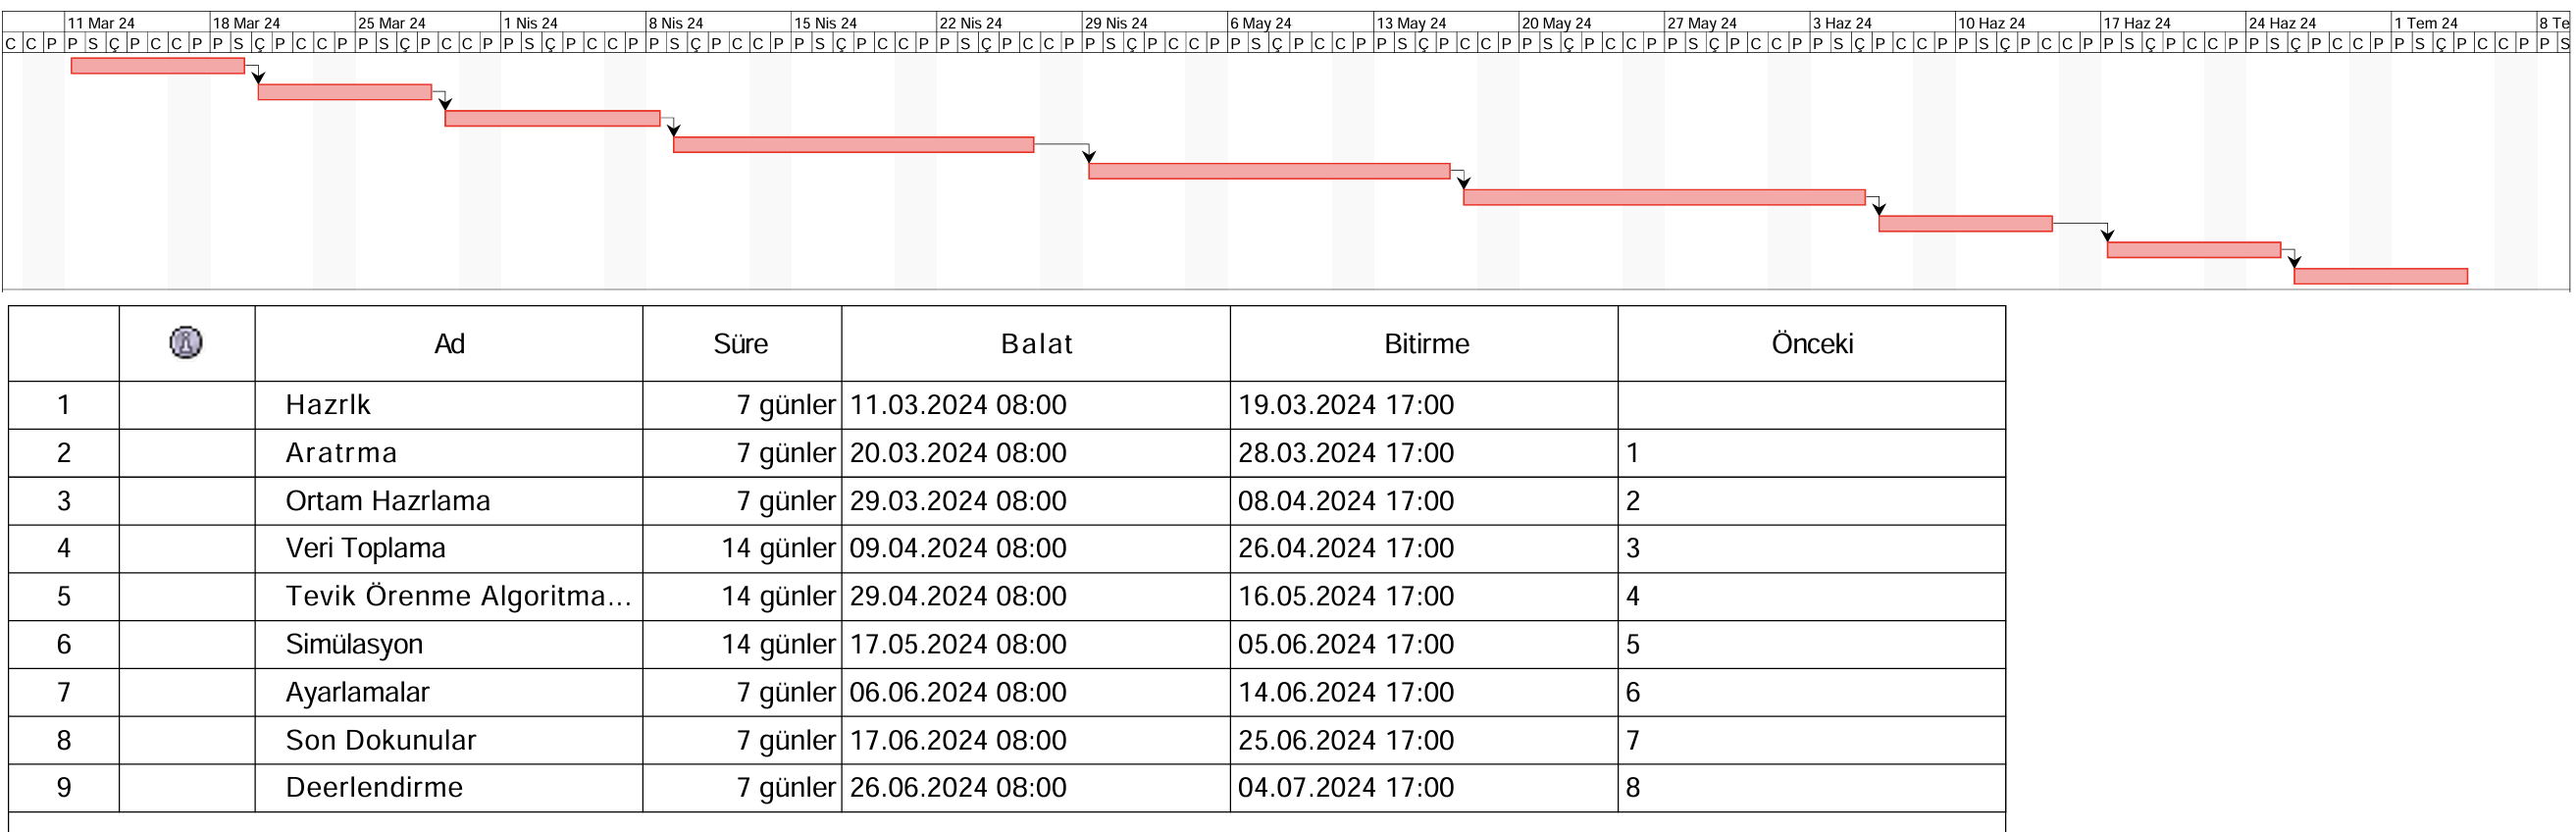
\includegraphics[angle=90, width=0.5\textwidth]{gantchart.png}

\newpage

\bibliographystyle{ieeetr}
\bibliography{atıf}

\textit{Train Donkey Car in Unity Simulator with Reinforcement Learning}, 2018.
\par
\url{https://github.com/flyyufelix/donkey_rl}

\end{document}

